\subsection{Controller}

Krasner and Pope defined an application's controller in \autocite{krasner-pope-88} as an interface to associate the components of the system (\emph{model and view}) and incoming events (\emph{such as event coming from input devices}). In other words, the controller component is responsible in defining the flow or sequence of a system based on an incoming event, routing commands to the appropriate model and updating the view in the process.
In this subsection, an analysis of the use cases listed on \textbf{TODO: ref to use cases} will be done, and consequentially a sequence of operations will be defined for each specific use case. An additional sequence will also be defined as a way complete the system and fulfill the requirements defined.  


\subsubsection{Customer Validation on a Registration Event}
 \label{subsection:regis}

\begin{figure}[!ht]
 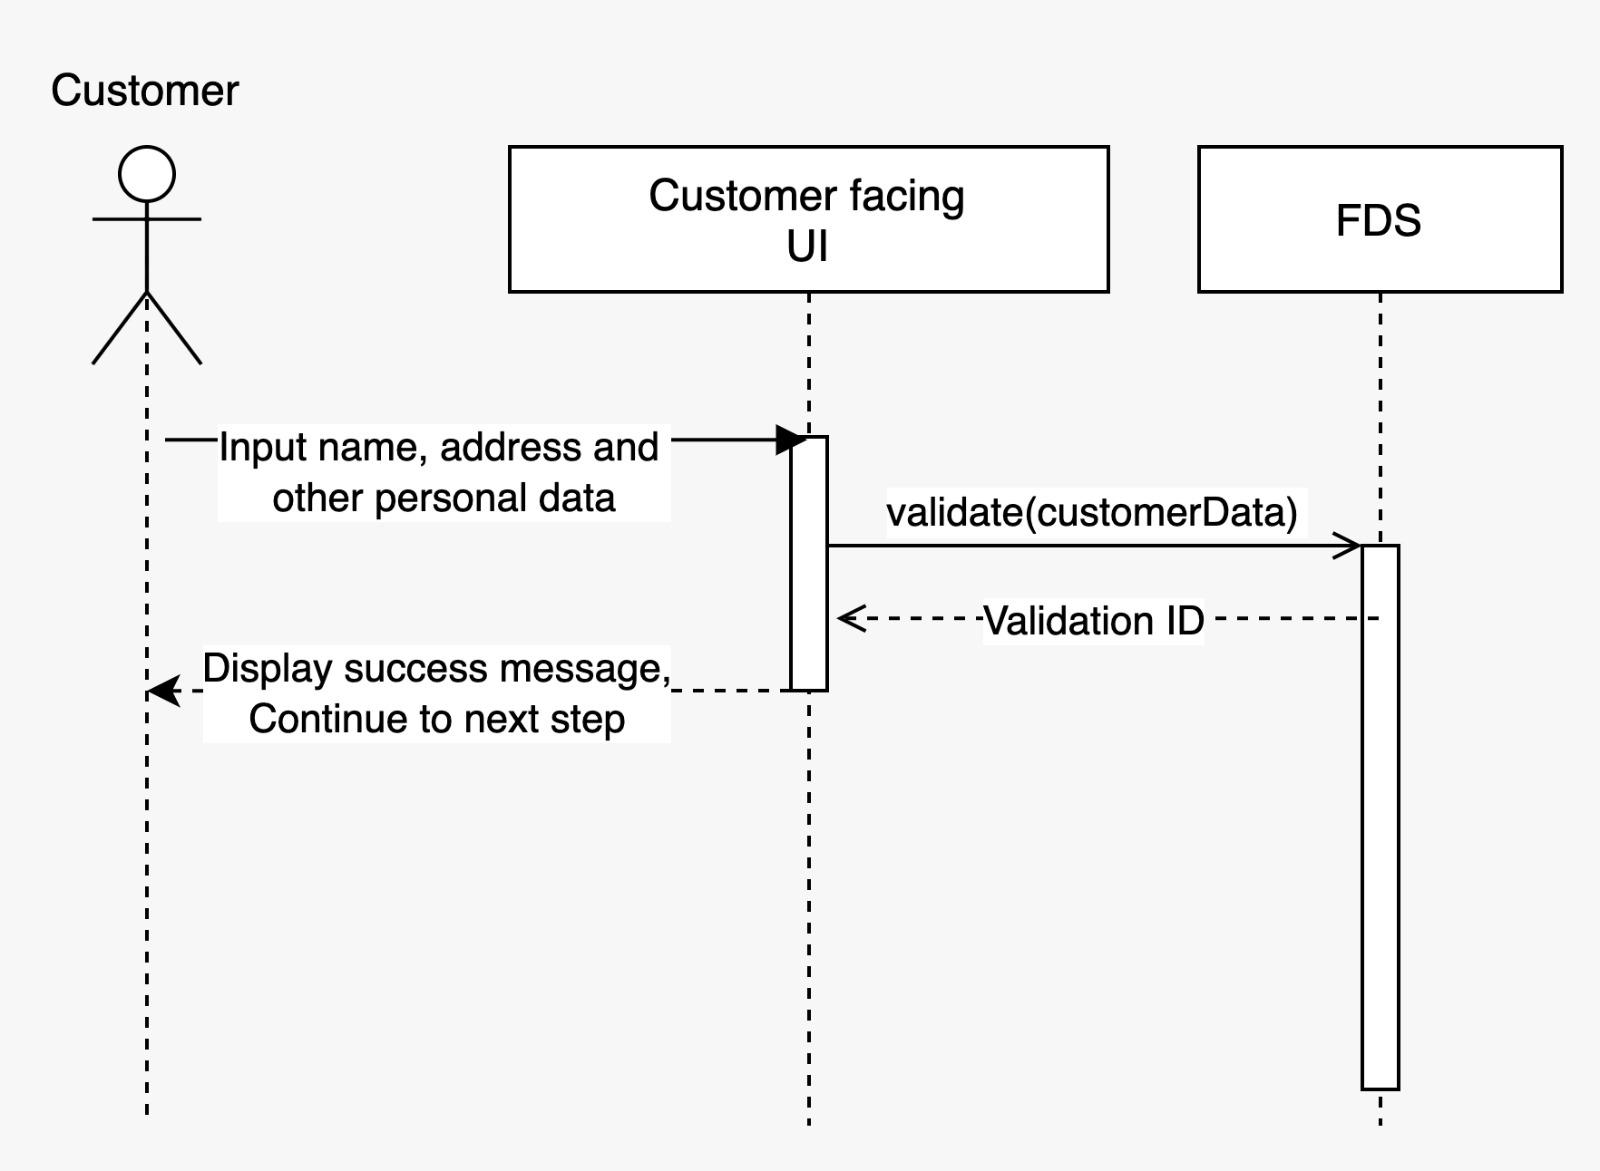
\includegraphics[width=\textwidth]{diagrams/sequence_registration.jpeg}
 \caption{System sequence diagram for a customer validation when a new customer is registered}
\end{figure}

A system sequence can be defined by analyzing the following use case:

\begin{quotation}
 \enquote{As a stakeholder, I want to verify customer, so that the company can have more confidence that the existing user base is trustworthy} 
\end{quotation}

One of the opportunity to do a verification process is during a new customer registration. Verifying a customer after each new registration might help the stakeholder to be more confident, that the user base is trustworthy and necessary actions can be taken as soon as possible to reduce the possible damage made in the future by fraudulent customers.
\begin{itemize}
 \item A new customer inputs his or her personal data to a customer facing UI and clicks the \emph{"Register"} button
 \item The customer facing UI makes an HTTP Post request to the FDS, containing the user's personal data on its request payload
 \item The FDS receives the HTTP request, and schedules a new validation process to be executed asynchronously
 \item The FDS responds to the HTTP request by returning a validation ID pointing to the scheduled validation process
 \item Customer facing UI shows a success message and continues registration to the next step while the validation process runs 
\end{itemize}


\subsubsection{Notification on Suspicious Cases}
 \label{subsection:seq-notification}

\begin{figure}[!h]
 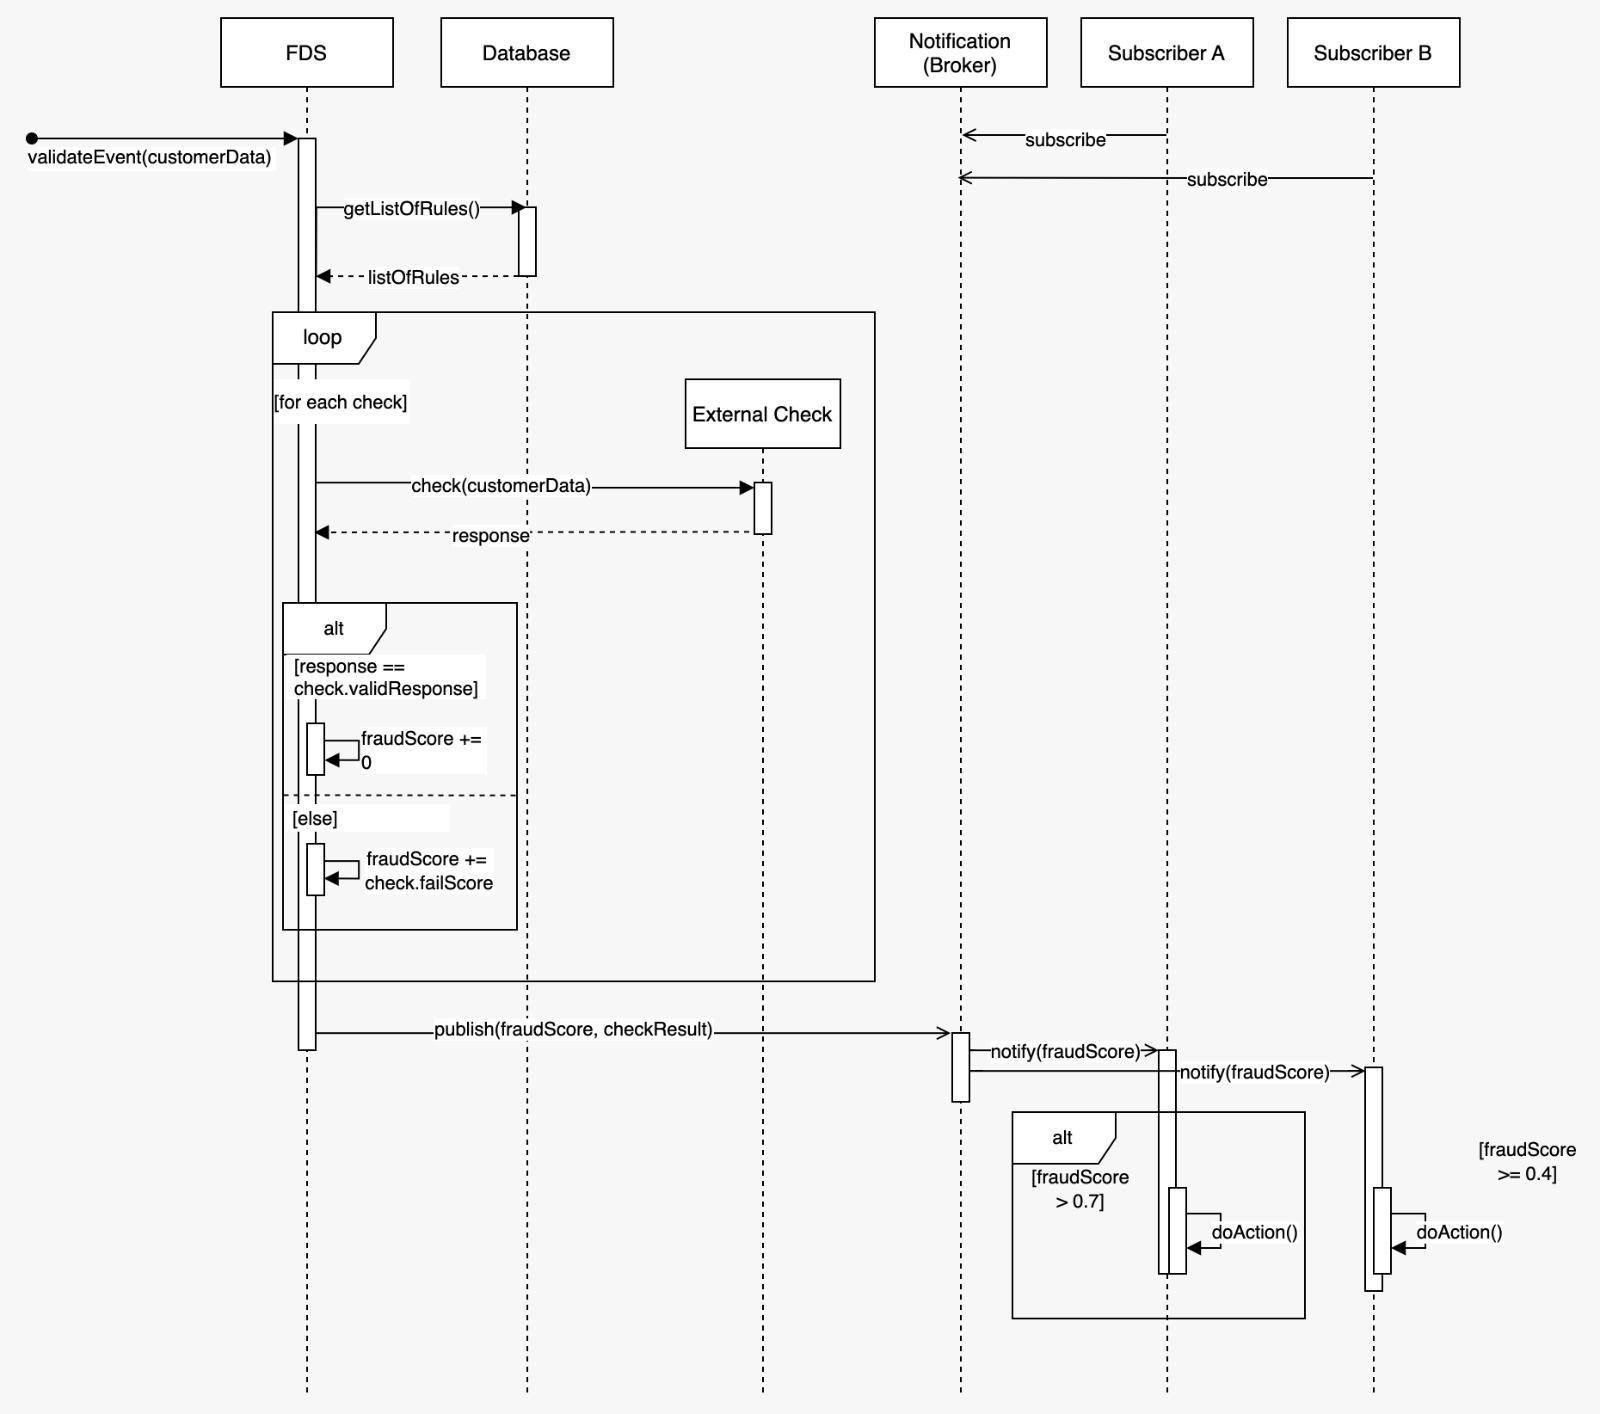
\includegraphics[width=\textwidth]{diagrams/sequence_notification.jpeg}
 \caption{System sequence diagram for notifications on suspicious cases}
\end{figure}

To fulfill the requirements listed on \textbf{TODO: Link Analysis}, a further examination of the following use case should be done:

\begin{quotation}
 \enquote{As an employee, I want to be notified when a user seems suspicious, so that I can do necessary actions accordingly} 
\end{quotation}

The FDS runs a rule evaluation by making an HTTP request to an external URL and comparing the HTTP response to the conditions listed on the validation rule. As working with external systems can sometimes be unpredictable and there is no guarantee that the external system has a fast response time, a validation process is run asynchronously, meaning that the FDS would not return the validation result with a resulting fraud score directly to the client when a validation process is scheduled. At the end of a validation process, the concerned parties might need some kind of notification on certain cases, to make sure actions required can be made as soon as possible. The following sequence illustrates the sequence of activities done by the system to validate a certain customer and sending a notification on its completion.

\begin{itemize}
 \item The FDS receives an HTTP request to schedule a validation process and responds by returning the ID of the validation process
 \item FDS retrieves a list of validation rules from the database
 \item FDS begins to initiate a validation process by setting the fraud score to 0 and looping through the list of validation rules for evaluation
 \item A validation rule will be evaluated by making an HTTP request to the external endpoint defined by the validation rule and evaluating its response according to the condition specified
 \item If the response matches all the conditions specified by the validation rule, the rule evaluation will be considered as a success and the fraud score will be incremented with 0. Otherwise, the rule evaluation will be considered as a failure and the fraud score will be incremented by the \emph{fail score} specified by the validation rule
 \item After the evaluation of all validation rules retrieved from the database is completed, the FDS publishes the validation result to an exchange hosted created the message broker
 \item The message consumers consume the message from the exchange and react accordingly\footnote{For example: sending an email notification if the fraud score exceeds 0.7.}
\end{itemize}


\subsubsection{Managing Validation Rules}
 \label{subsection:management}

\begin{figure}[!ht]
 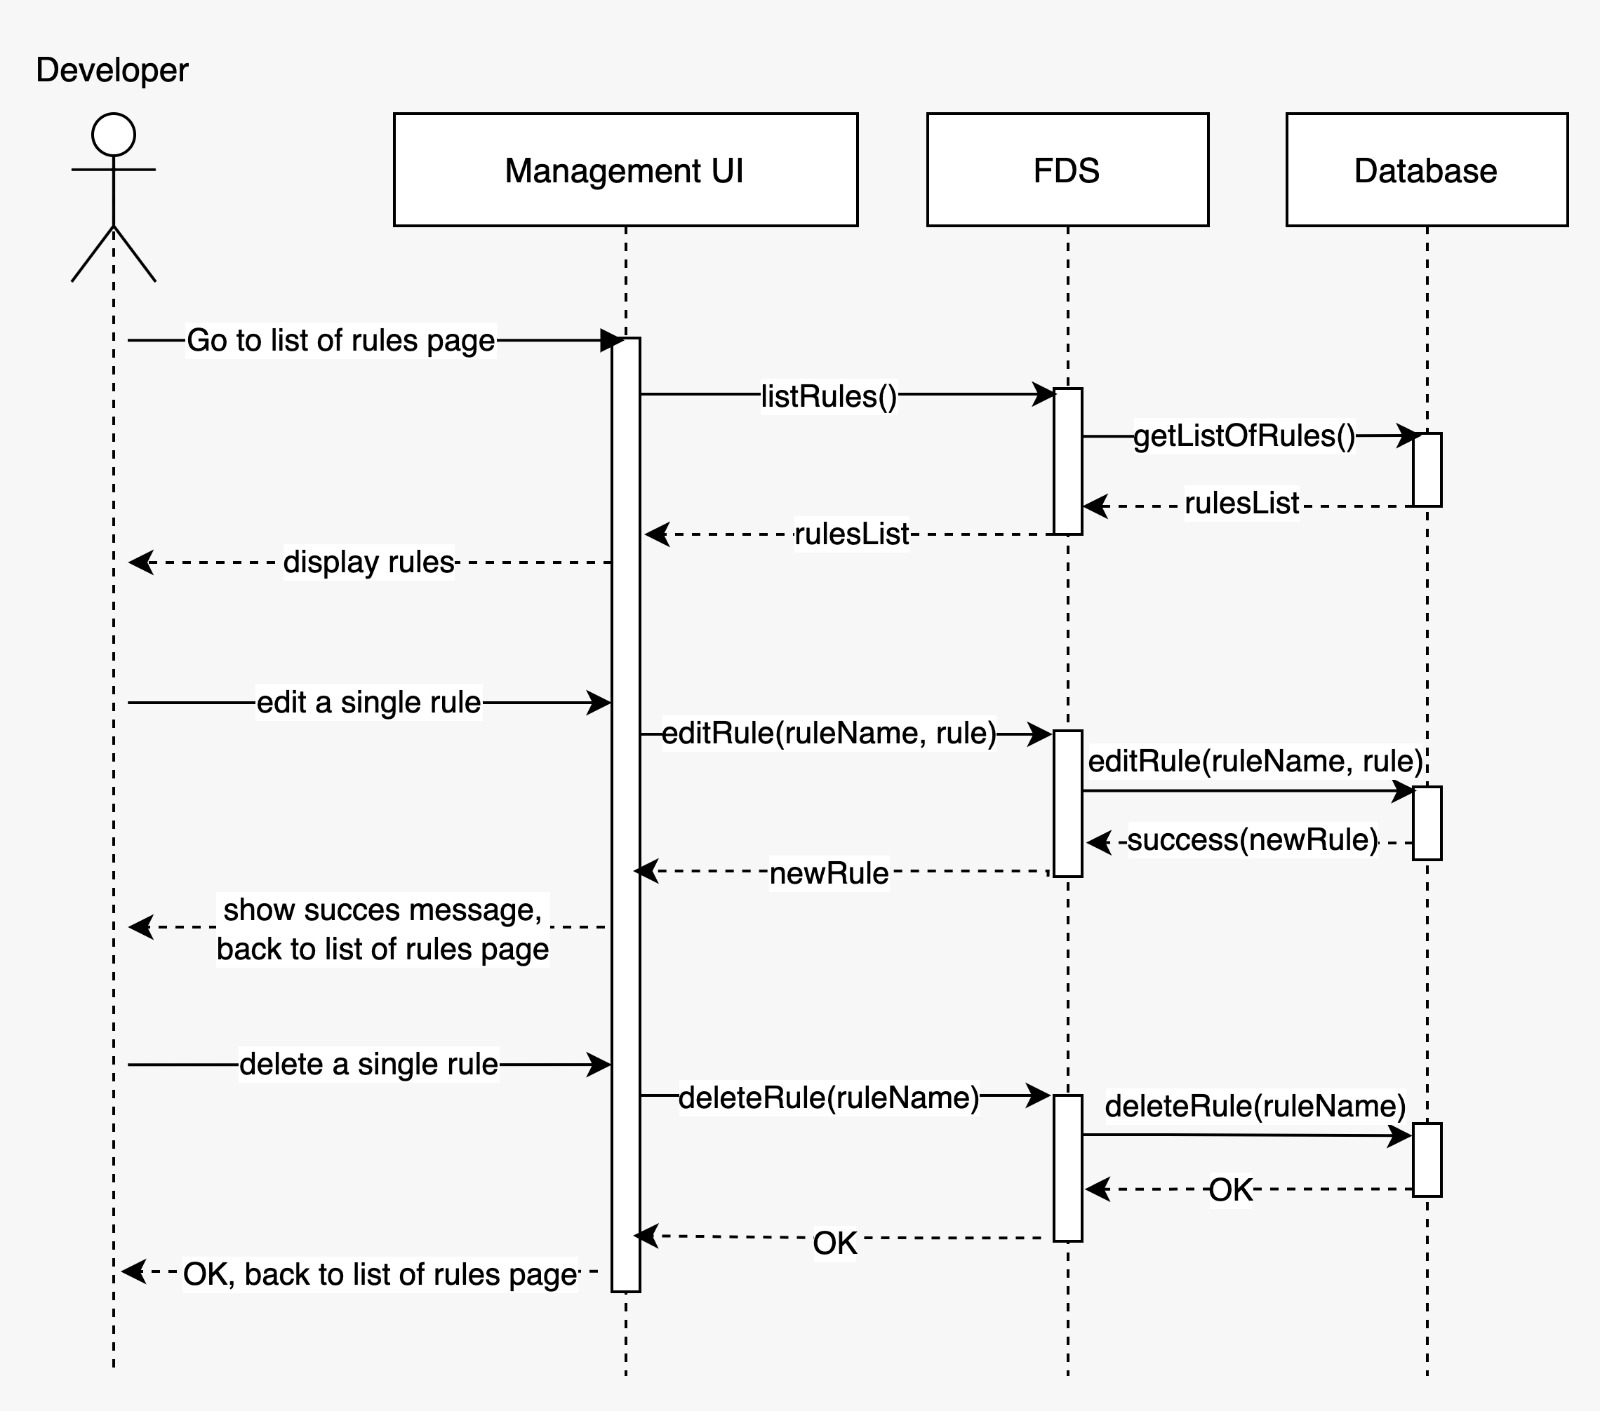
\includegraphics[width=\textwidth]{diagrams/sequence_management.jpeg}
 \caption{System sequence diagram for validation rules management}
\end{figure}

Another sequence can also be defined as a result of an analysis of the following use case:

\begin{quotation}
 \enquote{As an employee, I want to manage my own rule to validate users, so that I can use my expertise to find suspicious customers as efficiently as possible without the communication overhead with other teams} 
\end{quotation}

A possibility for each team to manage their own validation rules without being dependent to other teams is needed. By reducing the impediment in the process (having to consult other teams, communication overhead), every team can focus on generating validation rules that reflect a fraudulent customer as efficiently as possible, according to their own domain knowledge and expertise.

\begin{itemize}
 \item A user (e.g. Developer) can access the management UI and go to the page that displays a list of available validation rules
 \item The FDS retrieves a list of validation rules from the database
 \item User can click on a single rule and edit the rule
 \item The management UI makes an HTTP PUT\footnote{In \autocite[\enquote{9.6 PUT}]{http-rfc}, HTTP PUT method is described as a method to store or modify an entity, defined by the Request-URI} request to the database to edit an existing rule
 \item The FDS receives the HTTP request, modify the rule on the database and returns the edited rule as a response
 \item The management UI displays a success message and redirects user back to the list of rules page
 \item User can click on a single rule and delete the rule
 \item The management UI makes an HTTP DELETE\footnote{In \autocite[\enquote{9.7 DELETE}]{http-rfc}, HTTP DELETE method is described as a method to delete a resource on the host server, pointed by the Request-URI} request to the database to delete an existing rule
 \item The FDS receives the HTTP request and delete the rule on the database, returning a 204\footnote{In \autocite[\enquote{10.2.5 204 No Content}]{http-rfc}, the 204 status code should be used if the server fulfilled the request, but no data should be returned by the HTTP response} status code as an identifier of a successful operation
 \item The management UI displays a success message and redirects user back to the list of rules page
\end{itemize} 


\subsubsection{Validation Real-Time Progress}

\begin{figure}[!ht]
 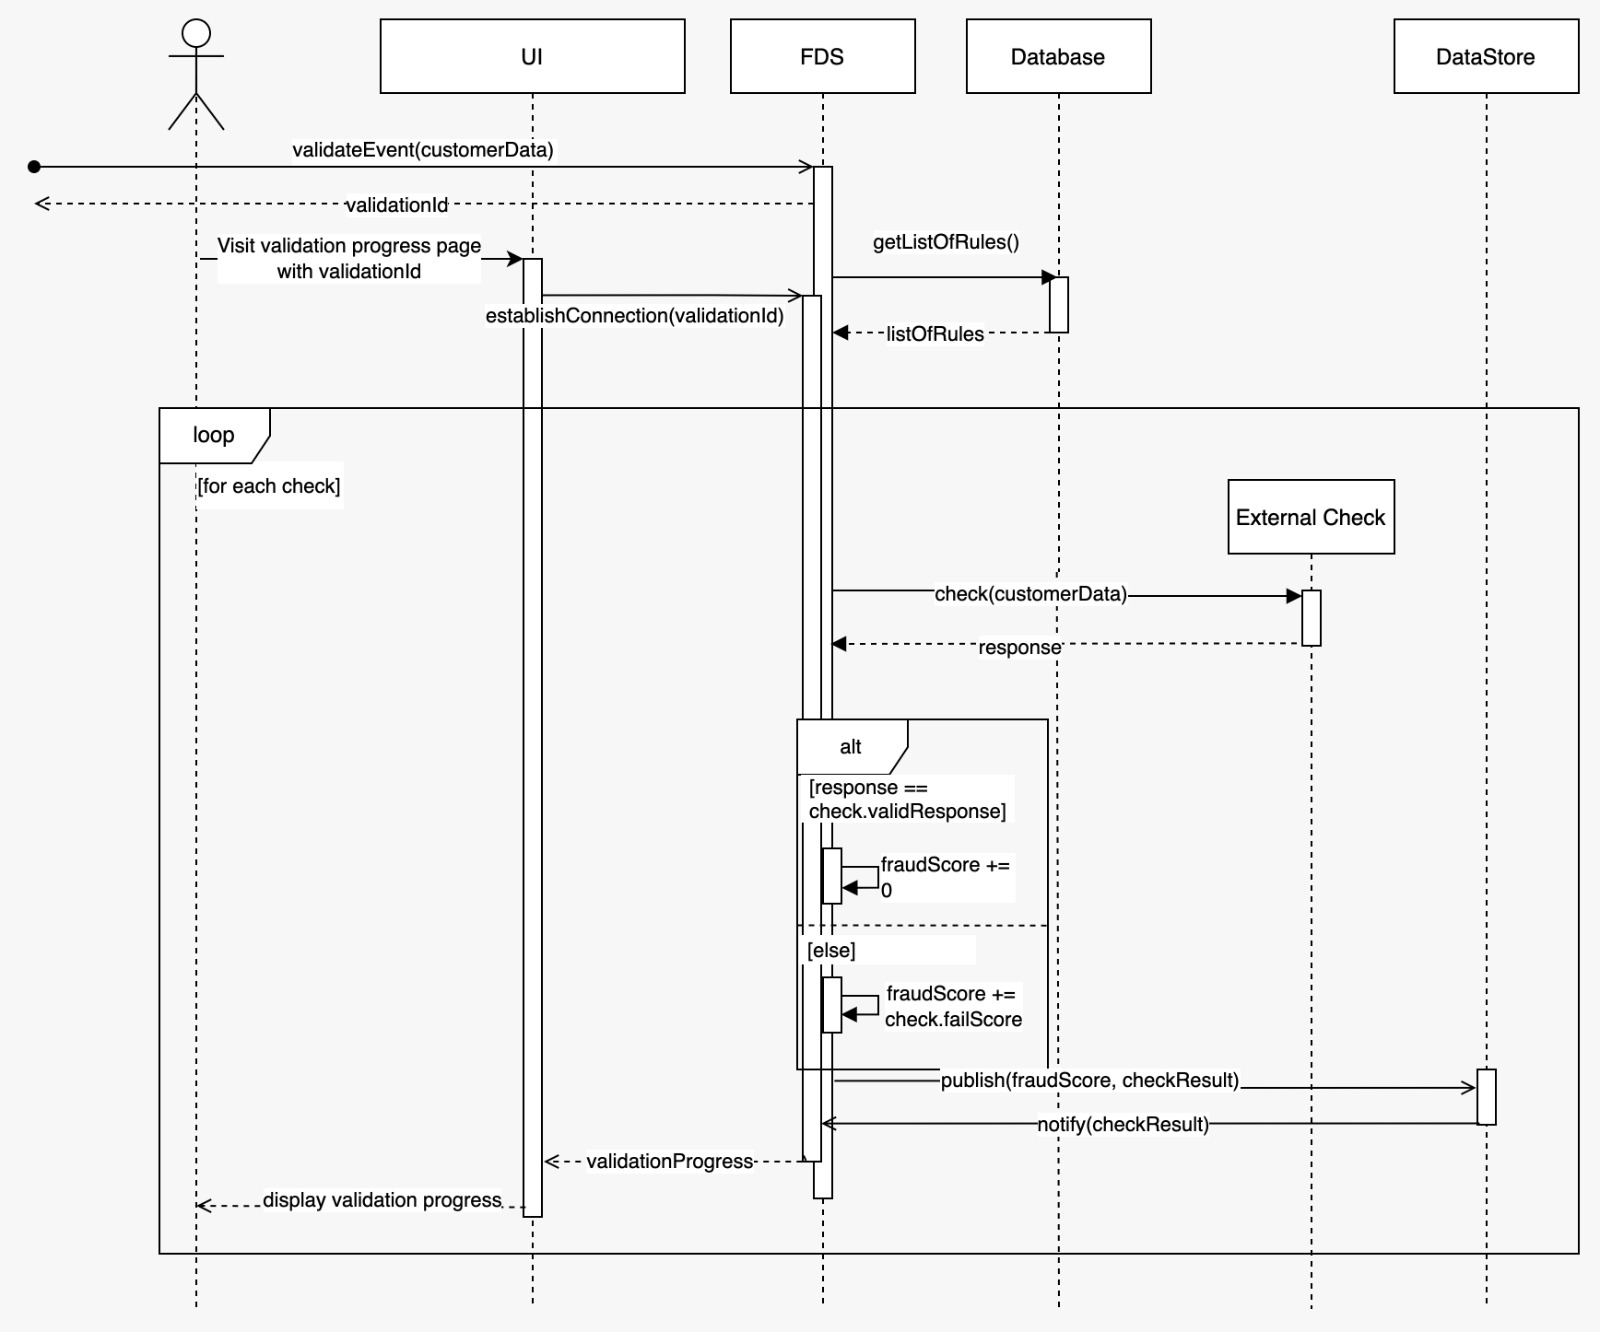
\includegraphics[width=\textwidth]{diagrams/sequence_pubsub.jpeg}
 \caption{System sequence diagram for validation rules management}
\end{figure}

Even though the user should receive a notification on certain cases, there might be certain cases where a user wants to intentionally monitor the progress of a validation result. To achieve such functionality, the user interface should establish a connection to the FDS, and receive notification whenever there is an update on the validation result. The sequence of such functionality will be as follows:

\begin{itemize}
 \item The FDS receives an HTTP request to schedule a validation process and responds by returning the ID of the validation process
 \item FDS retrieves a list of validation rules from the database and initiate the validation process
 \item A user visits the validation progress page with the returned validation 
 \item The user interface establishes a connection with the FDS subscription endpoint
 \item After each rule evaluation, the FDS stores the latest validation result to a data store\footnote{A data store in this context can be a caching memory or a simple class to store some temporary information}
 \item Every time the data store receives a new data, the user interface will get a notification and the latest result from the FDS subscription endpoint
 \item The user interface updates the view containing the latest validation result
\end{itemize}

